\section{Methodology}\label{methodology}
%
In this section we start by fixing the notation that we use for regression. We introduce more control-theoretic notation as we go along.
%
\subsection{Linear Least Squares}
Let $\designMat \in \mathbb{R}^{m \times n}$ be the design matrix, $\observations \in \mathbb{R}^{m}$ the vector of observations and  $\param \in \mathbb{R}^{n}$ the parameter vector to be estimated: $\designMat\param \approx \observations$. In this linear regression model $\residual = \observations - \designMat\param$ are the residuals that are to be minimized with respect to 2-norm~\cite{Golub80}
%
\begin{equation}
\begin{aligned}
\text{minimize} &\ \residual^{\mathrm{T}}\weightingMat\residual, \\
\text{subject to} &\ \observations + \residual \in \text{Range}(\designMat).
\end{aligned}
\label{lls}
\end{equation}
%
\noindent The weight matrix $\weightingMat$ is chosen to be positive definite and ideally should be the inverse of the covariance matrix $\covarRes$ of the residuals. The well-known \emph{normal equations} $\designMat^{\mathrm{T}}\weightingMat\designMat \param = \designMat^{\mathrm{T}} \weightingMat\observations$ provide the unique closed-form solution to this problem in case $\designMat$ is of full rank, $\text{rank}(\designMat) = n$. Solution to the normal equations can then be computed in a numerically stable way~\cite{Golub96} using e.g. QR decomposition methods. If the design matrix $\designMat$ is of low rank, pseudoinverse $\designMat^{\dagger}$ finds out of infinitely many solutions the minimum 2-norm solution $\hat{\param} = \designMat^{\dagger}\observations$ and can be computed using SVD. % this should be verified. [see Golub'96]

In case the design matrix $\designMat$ is numerically rank-deficient (i.e. its condition number is large), ridge regression (i.e. Tikhonov regularization) or truncation methods can be used to regularize (and hence to come up with a numerically stable estimate of) the parameter $\param$ in \eqref{lls}. Truncation can be applied conveniently with the pseudoinverse: invert the large singular values of $\designMat$ above a certain user-specified threshold $\threshold$ and truncate the rest to zero.

\subsection{Total Least Squares: an errors-in-variables model}
% shall we use multiple right hand sides?
% include weighting in the derivation?

Total Least Squares (TLS) is an errors-in-variables model that is applicable when the design matrix $\designMat$ is also not precisely known,
i.e., $(\designMat + \errorMat)\param = \observations + \residual$ for an unknown $\errorMat$ hopefully with small norm. An optimization procedure with diagonal weighting matrices $\weightingMat_{L} \in \mathbb{R}^{m \times m}$ and $\weightingMat_{R} \in \mathbb{R}^{n+1 \times n+1}$ minimizing both errors is a natural extension of \eqref{lls} under this model
%
\begin{equation}
\begin{aligned}
\text{minimize} &\ \| \weightingMat_{L} \begin{bmatrix} \errorMat & \residual \end{bmatrix} \weightingMat_{R} \|, \\
\text{subject to} &\ \observations + \residual \in \text{Range}(\designMat + \errorMat).
\end{aligned}
\label{tls}
\end{equation}
%
\noindent The singular-value decomposition (SVD) based solution to~\eqref{tls} for the Frobenius norm or the spectral norm is described in \cite{Golub80} \footnote{However in general \ref{tls} fails to have a solution. An example with low-rank design matrix can be found in \cite{Golub80}.} and relies on the Eckart-Young theorem. We show here for convenience the case where the weighting matrices $\weightingMat_{L}$ and $\weightingMat_{R}$ are identity. Rewriting $(\designMat + \errorMat)\param = \observations + \residual$ as  
%
\begin{equation}
\begin{aligned}
\begin{bmatrix} \designMat + \errorMat & \observations + \residual \end{bmatrix} \begin{bmatrix} \param \\ -1 \end{bmatrix} = 0, \\
\end{aligned}
\end{equation}
%
\noindent and using the Eckart-Young decomposition for a minimum Frobenius norm or spectral norm matrix $\begin{bmatrix} \hat{\errorMat} & \hat{\residual} \end{bmatrix}$% reference needed 
%

\begin{align}
\begin{bmatrix} \designMat & \observations \end{bmatrix} = \begin{bmatrix} \leftEigenvector_{X} & \vec{u}_{y} \end{bmatrix} \begin{bmatrix} \vec{\Sigma}_{X} & 0 \\ 0 & \sigma_{y} \end{bmatrix} \begin{bmatrix} \rightEigenvector_{XX} & \vec{v}_{Xy} \\ \vec{v}_{yX} & v_{yy} \end{bmatrix}^{\mathrm{T}}, \label{eckart1} \\
\begin{bmatrix} \designMat + \hat{\errorMat} & \observations + \hat{\residual} \end{bmatrix} = \begin{bmatrix} \leftEigenvector_{X} & \vec{u}_{y} \end{bmatrix} \begin{bmatrix} \vec{\Sigma}_{X} & 0 \\ 0 & 0 \end{bmatrix} \begin{bmatrix} \rightEigenvector_{XX} & \vec{v}_{Xy} \\ \vec{v}_{yX} & v_{yy} \end{bmatrix}^{\mathrm{T}} \label{eckart2}.
\end{align}
% 
\noindent After subtracting \eqref{eckart2} from \eqref{eckart1} and manipulating we get
%
\begin{align}
\hat{\param}_{tls} &= -\frac{\vec{v}_{Xy}}{v_{yy}}, \label{tls1} \\
\hat{\errorMat} &= \leftEigenvector_{X} \vec{\Sigma}_{X} \rightEigenvector_{XX}^{\mathrm{T}} - \designMat. \label{tls2}
\end{align}

\noindent The SVD solution nicely separates the parameter estimate $\hat{\param}$ from the \emph{latent matrix} estimate $\hat{\latentMat} = \designMat + \hat{\errorMat} = \leftEigenvector_{X} \vec{\Sigma}_{X} \rightEigenvector_{XX}^{\mathrm{T}}$. See Figure~\ref{Figure1} for an illustration in one-dimensional regression. The case for multiple right-hand sides (i.e. $\observations \in \mathbb{R}^{n \times k}, k > 1$) and diagonal weighting matrices is given in \cite{Golub96}. Further extensions including partial, structured, and truncated TLS can be found in \cite{VanHuffel91}. Note that these extensions often lack a closed-form solution and must be iteratively computed.
% alternating projections?
% more citations are necessary!
% mention that we are extracting a latent dynamics matrix F_est = F + E!
Pseudocode for a general truncated total least squares algorithm implementing an SVD solution is given in Algorithm~\ref{alg1}. Notation is adapted slightly for the general case. The latent matrix estimation step is made explicit. % refer to latent matrix estimation (PCA?) literature.
%
\begin{figure}
\centering
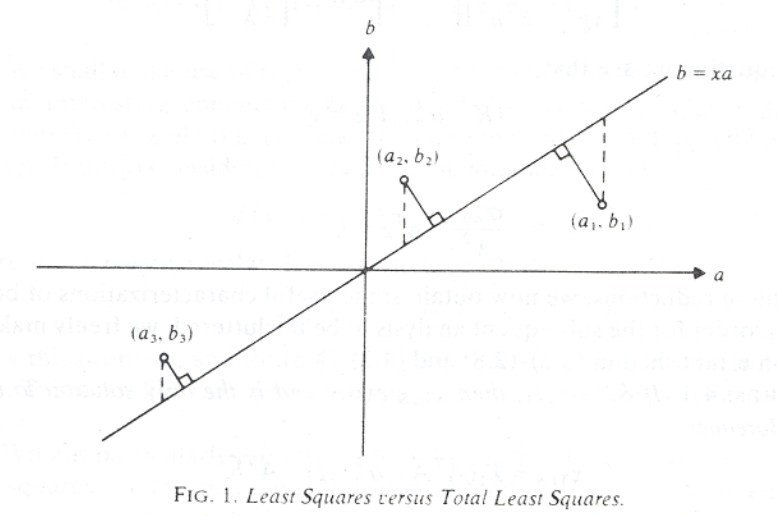
\includegraphics[width=0.4\textwidth]{LSvsTLS.jpg}%
\caption{Comparison between least squares and total least squares in the one dimensional estimation setting, taken from \cite{Golub80}. Least Squares minimizes the sum of the squared vertical distances from observations to the regression line. Total Least Squares is also known as orthogonal regression in 1D and minimizes instead the sum of the squared perpendicular distances.}
\label{Figure1}
\end{figure}
%
%
\begin{algorithm}[tb]
   \caption{Truncated Total Least Squares}
   \label{alg1}
\begin{algorithmic}
   \STATE {\bfseries Input:} $\threshold > 0$, $\designMat$, $\fullObs = \begin{bmatrix} \observations_1 & \observations_2 & \ldots & \observations_k \end{bmatrix}$, diagonal $\weightingMat_{L}$, $\weightingMat_{R} = \begin{bmatrix} \weightingMat_{R1} & \weightingMat_{R2}\end{bmatrix}$.
   \STATE Compute SVD solution $\leftEigenvector \vec{\Sigma} \rightEigenvector^{\mathrm{T}}$ to $\weightingMat_{L}\begin{bmatrix} \designMat & \fullObs \end{bmatrix}\weightingMat_{R}$.
   \STATE Estimate parameter $\hat{\fullParam} = -\weightingMat_{R1}\vec{V}_{XY}\vec{V}_{YY}^{\dagger}\weightingMat_{R2}^{-1}$.
   \STATE Estimate latent matrix $\hat{\latentMat} = \leftEigenvector_{X} \vec{\Sigma}_{X} \rightEigenvector_{XX}^{\mathrm{T}}$.
\end{algorithmic}
\end{algorithm}
%
%
\subsection{Iterative Learning Control with Total Least Squares}\label{ilcTLS}
%
In Iterative Learning Control (ILC) the goal is to minimize deviations from a fixed reference trajectory $\traj(t), \ 0 \leq t \leq~T$ in state space $\state \in S \subset \mathbb{R}^{p}$ when the system to be controlled is subject to unknown repeating disturbances and model mismatch \cite{Bristow06}. As opposed to other adaptive control or reinforcement learning approaches~\cite{NguyenTuong11} in ILC usually the feedforward control inputs to the system $\sysInput_k(t)$ are adjusted after each iteration $k = 1, 2, \ldots$ is completed and the resulting deviations $\error_k(t) = \state_k(t) - \traj(t)$ from the desired trajectory are observed. % references to adaptive control literature?

Consider a general nonlinear dynamical system governed by the differential equation
%
\begin{align}
\dot{\state} &= \dynamics(\state,\sysInput), \label{dynamics} \\
\dot{\state} &= \dynamicsNominal(\state,\sysInput) + \dist(\state,\sysInput). \label{dynamicsNom}
\end{align}
%
% reference to other nonlinear approaches to ILC?
\noindent Assume that the nominal model $\dynamicsNominal$ is all we know about the system in \eqref{dynamics}. Nonlinear approaches to ILC mostly consider linearizations of \eqref{dynamicsNom} around the trajectory $\traj(t)$ and nominal inputs $\trjInput(t)$.
% citation needed
Discretizing and stacking the linear time varying matrices obtained, we get the following \emph{lifted-form} approximation of the underlying dynamics
%
\begin{equation}
\begin{aligned}
\error_k \approx \systemMat \sysInput_k + \linDist,
\end{aligned}
\label{approxModel}
\end{equation}
%
\noindent where the model matrix $\systemMat$ has a block lower-diagonal structure, and is composed of the submatrices
%
\begin{equation}
\begin{aligned}
\vec{F}_{(i,j)} &= \left \{
\begin{array}{cc}
\vec{A}_{i-1}\ldots \vec{A}_j \vec{B}_{j-1}, & j < i, \\ 
\vec{B}_{j-1}, & j = i, \\
\vec{0}, & j > i. 
\end{array} \right.
\end{aligned}
\label{Fmatrix}
\end{equation}

\noindent Matrices $\vec{A}_j$ and $\vec{B}_j$ are linearizations of the nominal model $\dynamicsNominal$ around the discrete trajectory points $\traj_j$ and nominal inputs $\vec{\nu}_j$ respectively. Conventional ILC algorithms using such a linearized model compute at each iteration the feedforward compensation signals $\sysInput = (\sysInput_1^{\mathrm{T}}, \ldots, \sysInput_N^{\mathrm{T}})^{\mathrm{T}}$ added to the nominal inputs $\trjInput = (\trjInput_1^{\mathrm{T}}, \ldots, \trjInput_N^{\mathrm{T}})^{\mathrm{T}}$ to drive error $\error = (\error_1^{\mathrm{T}}, \ldots, \error_N^{\mathrm{T}})^{\mathrm{T}}$ to its theoretical minimum (ideally zero). For example, the ILC algorithm utilizing plant inversion with pseudoinverse 
% reference needed
computes the updates using % ref needed
% 
%
\begin{equation}
\begin{aligned}
\sysInput_{k} = -\systemMat^{\dagger}\linDist_{k},
\end{aligned}
\label{pseudoinverseILC1}
\end{equation}
%
\noindent where $\linDist_{k}$ is estimated from \eqref{approxModel} using the last iteration $k-1$, i.e., $\linDist_{k} \approx \systemMat \sysInput_{k-1} - \error_{k-1}$. When the system matrix $\systemMat$ is of full rank, we get the following model-based ILC update law 
%
\begin{equation}
\begin{aligned}
\sysInput_{k+1} = \sysInput_{k} - \systemMat^{\dagger}\error_{k}.
\end{aligned}
\label{pseudoinverseILC2}
\end{equation}
%
\noindent The command for computing the pseudoinverse in MATLAB with truncation parameter $\epsilon$ is \emph{pinv}$(\designMat,\epsilon)$ where the singular values of $\designMat$ less than $\epsilon$ are treated as zero. 

The compensations in \eqref{pseudoinverseILC2} are computed using the approximate model in \eqref{approxModel} and should be reconsidered. In particular, it is not enough to state that the control inputs will eventually converge to a steady-state value, as is often done when proving the \emph{stability} of ILC algorithms. For practical and for safety purposes one needs to also ensure that the errors incurred along the trajectory at each iteration are decreasing, under a particular vector norm. This is studied in the ILC literature under \emph{monotonic convergence}~\cite{Bristow06}. 

Satisfying the monotonic convergence criterion when the dynamics involves unknown perturbations 
%
\begin{equation}
\begin{aligned}
\error_k = (\systemMat + \errorMat_k)\sysInput_k + \linDist_k,
\end{aligned}
\label{exactModel}
\end{equation}
%
\noindent requires a more cautious ILC update. Using Total Least Squares, combining \eqref{pseudoinverseILC2} and \eqref{tls} we derive $\alg$
%
\begin{align}
\sysInput_{k+1} &= \sysInput_{k} - \delta \sysInput_{k}, \label{tlsilc1} \\ 
\delta \sysInput_{k}, \ \hat{\errorMat}_k &= \arg\min \|\begin{bmatrix}\errorMat_k & \residual_k \end{bmatrix} \|_{2}, \label{tlsilc2} \\
\text{subject to} &\ (\systemMat + \errorMat_k)\delta \sysInput_k = \error_k + \residual_k \label{tlsilc3}.
\end{align}
%
\noindent This new ILC law is stated in algorithmic form in Algorithm~\ref{alg2}.
%
\begin{algorithm}[tb]
   \caption{Cautious ILC Algorithm $\alg$}
   \label{alg2}
\begin{algorithmic}
   \STATE {\bfseries Input:} $\threshold > 0$, horizon $\numSteps$, diagonal $\weightingMat_{L}$, $\weightingMat_{R} = \begin{bmatrix} \weightingMat_{R1} & \weightingMat_{R2}\end{bmatrix}$.
   \STATE Form $\vec{F}$ using $\vec{A}$, $\vec{B}$ matrices up to horizon $\numSteps$
   \STATE Initialize $k = 0$, $\sysInput_0 = \trjInput$
   \REPEAT 
   	   \STATE Apply inputs $\sysInput_{k}$ and observe errors $\error_{k}$
	   \STATE Compute SVD solution $\leftEigenvector \vec{\Sigma} \rightEigenvector^{\mathrm{T}}$ to $\weightingMat_{L}\begin{bmatrix} \systemMat & \error_k \end{bmatrix}\weightingMat_{R}$.
	   \STATE Update inputs $\sysInput_{k+1} = \sysInput_{k} - \weightingMat_{R1}\vec{V}_{XY}\vec{V}_{YY}^{\dagger}\weightingMat_{R2}^{-1}$.
   \UNTIL{$\error_k \leq \error_{\infty} + \threshold$}
\end{algorithmic}
\end{algorithm}
%